\section{Framework}
\label{sec:frame}
We first introduce the procedure to extract positive events and their intervals from microblogs.
Based on this procedure,
we present a statistical model to depict the relationship between positive events and adolescents' stress-buffering patterns through three groups of content and behavioral measures.
%Finally, a none-liner time series model was proposed to combine stress-buffering patterns into future stress prediction.

\subsection{Discovery of Positive Events from Microblogs}
\label{sec:frame1}
Let $u$ = $[type,\{doer, act,$ $description\}]$ be a positive event,
where the element \emph{doer} is the subject who performs the \emph{act},
and \emph{description} is the list of key words related to $u$.
According to psychological scales ~\citep{Jun2008Influence,hassles},
positive events for adolescents mainly focus on six dimensions:
$\mathbb{U} =\{$ 'entertainment', 'school life', 'romantic relationships',
'peer relationships', 'self-cognition', 'family life'$\}$.
We constructed our lexicon for six-dimensional positive events from two sources.
The basic positive words are selected from the psychological lexicon C-LIWC
(expectation, joy, love, and surprise)~\citep{Tausczik2010The}.
Then, we built six topic lexicons by expanding basic positive words from the adolescents' microblogs,
containing 452 phrases in 'entertainment',
273 phrases in 'school life',
138 phrases in 'romantic relationships',
91 phrases in 'peer relationships',
299 phrases in 'self-recognition' and 184 phrases in 'family life', for a total 2,606 phrases.
Examples are shown in Table \ref{tab:topicWords}.
Additionally, we labeled \emph{doer} words (i.e., \emph{teacher}, \emph{mother},
\emph{I} and \emph{we}) in positive lexicons.

\begin{table*}
\centering
\caption{\small{Examples and statistics for topic phrases in the six-dimensional lexicons of positive events.}}
\label{tab:topicWords}
\small{
\begin{tabular}{lll}
\toprule
Dimension & Example words & total \\ \midrule
entertainment  & hike, travel, celebrate, dance, swimming, ticket, shopping, air ticket, theatre, party, Karaoke,& 452\\
                      & self-driving tour, game, idol, concert, movie, show, opera, baseball, running, fitness, exercise & \\
school life    & reward, come on, progress, scholarship,admission, winner, diligent, first place, superior & 273\\
				      & hardworking, full mark,  praise, goal, courage, progress, advance, honor, collective honor& \\
romantic  relationships&  beloved, favor, guard, anniversary,  concern, tender, deep feeling, care, true love, promise, & 138\\
				      & cherish, kiss, embrace, dating, reluctant, honey, sweetheart, swear, love, everlasting, goddess &\\
peer relationships  & listener, company, pour out, make friends with, friendship, intimate, partner, team-mate, brotherhood& 91\\
self-cognition & realize, achieve, applause, fight, exceed, faith, confidence, belief, positive, active, purposeful & 299\\
family life    & harmony, filial, reunite, expecting, responsible, longevity, affable, amiability, family, duty & 184\\
\bottomrule
\end{tabular}}
\end{table*}

\begin{table}[h]
\begin{center}
\caption{\small{Examples of automatically extracted positive events from the adolescents' microblogs.}}
\small{
\begin{tabular}{|l|} \hline
I am really looking forward to the spring outing on Sunday. \\
(doer:\emph{I}, act:\emph{looking forward}, description:\emph{spring outing})\\\hline
My holiday is finally coming [smile]. \\
(doer:\emph{My holiday}, act:\emph{coming}, description:\emph{[smile]})\\\hline
First place on my lovely math exam!!! In memory of it.\\
(description:\emph{first place, math, exam, memory})\\\hline
You are always here for me like sunshine. \\
(doer:\emph{You}, description:\emph{sunshine})\\\hline
Thanks to all my dear friends for hosting the party. Happiest\\
birthday!!! (doer:\emph{friends}, act:\emph{thanks}, description:\emph{party, birthday})\\\hline
I know my mom is the one who will support me forever, no matter \\
when and where. (doer:\emph{mom}, act:\emph{support})\\ \hline
Expecting tomorrow' Adult Ceremony[Smile][Smile]~~\\
(act: \emph{expecting}, description:\emph{Adult Ceremony})\\\hline
\end{tabular}}
\label{tab:uplifts}
\end{center}
\end{table}

\subsubsection{Linguistic Parser Model}
Positive events were identified through a Chinese natural language processing platform \citep{Che2010}.
For each post, after word segmentation, we parsed each sentence to find its linguistic structure
and then matched the main linguistic components with positive topic lexicons in each dimension.
A linguistic parser model was applied to identify the central verb of the current sentence, namely, the \emph{act}.
It constructed the relationship between the central verb and corresponding \emph{doer} and \emph{description} elements.
By searching these elements in positive topic lexicons,
the existence of positive events was identified.
Due to the sparsity of posts, the element \emph{act} might be empty.
\emph{Descriptions} were collected by searching all nouns, adjectives and adverbs.
Examples of positive events extracted from the adolescents' microblogs are listed in Table \ref{tab:uplifts}.
For example, the post 'Thanks all my dear friends for hosting the party. Happiest birthday!!!'
was processed as \emph{doer='friends', act = 'expecting', description = 'party'},
and \emph{type = 'entertainment'}.

\subsubsection{Impact Intervals of Positive Events}
\label{subsec:interval}
We followed and extended the method in~\citep{Li2017Analyzing} to identify the impact interval of each positive event to further study its stress-buffering pattern.
The target interval was identified in three steps.

Step1: Positive events, stressor events and filtered-out candidate intervals were extracted.
For each candidate interval,
we set its length to more than 3 days and a maximum gap of 1 day between two neighboring stressful days.
Since the stress series detected from the microblogs were discrete points,
the locally weighted regression~\citep{Cleveland1988Locally} method was adopted to highlight the characteristics of the stress curve.

Step2: Intervals were judged as stressful or not through hypothesis testing.
A Poisson-based probability model was adopted to measure how confident we are that the current interval was a stressful interval.
Here,
the stressful posting rates under stressful $\lambda_1$ and normal conditions $\lambda_0$ were modeled
as two independent Poisson processes:
\begin{equation}
Pr[N=n|\lambda_i]=\frac{e^{-\lambda_i T}{(\lambda_i T)}^n}{n!}
\end{equation}
where $i\in\{0,1\}$ and $n=0,1,\cdots,\infty$.
We expected that $\lambda_1 > \lambda_0$ and measured the probability as $P(\lambda_1>\lambda_0|N_1, T_1, N_0, T_0)$,
where $N_1$ and $N_0$ are the numbers of stressful posts
and $T_1$ and $T_0$ are the time durations corresponding to $\lambda_1$ and $\lambda_0$, respectively.
Without loss of generality, we assumed a Jeffreys noninformative prior on $\lambda_1$ and $\lambda_0$
and inferred the posterior distribution $P(\lambda_1|N_1)$ and $P(\lambda_0|N_0)$ according to Bayes' Rule.
Thus, for current interval $I_1$ and historical normal interval $I_0$,
the quantified probability $\beta = P(\lambda_1>\lambda_0|I_1,I_0)$ $\in (0,1)$
indicated confidence in whether $I_1$ was a stressful interval.

Step 3: The stressful intervals were divided  into an SI set and a U-SI set.
For a detected stressful interval $I = <t_1,\cdots,t_n>$,
we considered the temporal order between $I$ and any detected positive event $u$ occurring at time point $t_u$ in three cases:
\begin{itemize}
\item[1)] If the positive event $u$ occurred during the stressful interval, i.e., $t_u \in [t_1,t_n]$,
the positive interval $I$ was judged as $I \in U-SI$.
\vspace{-0.3cm}
\item[2)] If the positive event occurred near a stressful interval,
the probability that it had an impact on the current stressful interval was considered.
Here, the gap between $t_u$ and $I$ is limited to $\xi$, i.e.,
if $t_u \in [t_{1}-\xi, t_1)\cup(t_{n},t_{n}+\xi]$, then $I \in U-SI$.
If a stressful interval satisfies none of the above conditions, we classify it into the SI set.
\vspace{-0.3cm}
\item[3)] Other stressful intervals were classified into the U-SI set.
\end{itemize}

\subsection{Hypothesis Test for the Relationship Between Positive Events and Adolescents' Stress-buffering Patterns}
\label{sec:frame2}
We formulated the relationship between positive events and adolescents' stress-buffering patterns
as a comparison problem between two sets of stressful intervals: the SI set and the U-SI set.
Each interval was modeled as a multidimensional vector depicting microblogging characteristics of the current adolescent.
Specifically, a multivariate two-sample hypothesis test~\citep{Li2017Correlating,Johnson2012Applied} was adopted to model such a relationship.
The basic idea was to determine whether the multidimensional points (i.e., the stressful intervals)
in SI and U-SI were under different statistical distributions.
Assuming the data points in SI and U-SI were randomly sampled from distribution $F$ and $G$, respectively,
then the hypothesis can be denoted as follows:
\begin{equation}
H_0: F = G \quad versus \quad H_1: F \neq G.
\end{equation}
Under such a hypothesis,
$H_0$ indicates that points in SI and U-SI follow a similar distribution,
while $H_1$ means points in SI and U-SI follow statistically different distributions,
namely positive events had obvious stress-buffering effects.

\subsubsection{Statistical Model of the Stress-buffering Effect}
\begin{figure*}
\centering
\includegraphics[width=\linewidth]{figs/gray/stress.eps}
\caption{\small{Comparing stress change modes during stressful intervals in two situations:
1) intervals affected by positive neighboring events (U-SI) and
2) no positive events occurred nearby (SI).
$P_{1-6}$=\{school life, romantic relationships, peer relationships, self-cognition, family life, entertainment\},
$E_{1-5}$=\{school life, romantic relationships, peer relationships, self-cognition, family life\}.}}
\label{fig:stress}
\end{figure*}
We used a K-nearest-neighbor-based method~\citep{Schilling1986Multivariate}
to judge the existence of a significant difference between set SI and set U-SI.
For simplification, we used the symbol $A_1$ to represent set SI and $A_2$ to represent set U-SI.
For each point $\ell_{x}$ in the two sets,
we expected its top-k similar points to belong the same set of $\ell_x$.
The Euclidean distance was adopted to calculate the distance of structured points here.
For each point $\ell x \in A=A_1\bigcup A_2$,
let $\textbf{D}^y$ be the feature vector of $\ell_x$ and $NN_r(\ell_x,A)$ be the function to find the $r-$th nearest neighbor of $\ell_x$.
The $r$-th nearest neighbor of $\ell_x$ is denoted by:
\begin{equation}
\begin{aligned}
& NN_r(\ell_x,A) = \{y | min\{||\textbf{D}^x-\textbf{D}^y ||_2\}, y\in(A/\ell_x)\} &
\end{aligned}
\end{equation}
Let $I_r(\ell_x,A1,A2)$ be the function denoting whether the $r$-th nearest neighbor was in the same set as $\ell_x$:
\begin{equation}
I_r(\ell_x,A_1,A_2) =
\left\{ \begin{array}{ll}
1, \quad if \ell_x \in A_i  \&\& NN_r(\ell_x,A)\in A_i,\\
0, \quad otherwise
\end{array}
\right.
\end{equation}
Let $T_{r,n}$ denote the proportion that pairs containing two points from the same set among all pairs formed by $\ell_x \in A$ and its $k$ nearest neighbors:
\begin{equation}
T_{k,n}= \frac{1}{n\times k}\sum_{i=1}^{n}\sum_{j=1}^{k}I_j(x,A_1,A_2)
\end{equation}
The value of $T_{k,n}$ showed how differently the points in the two testing sets (SI and U-SI) performed.
If the value of $T_{r,n}$ was close to $1$,
then the two underlying distributions $F$ and $G$ for $SI$ and U-SI were significantly different,
indicating current positive events had an obvious stress-buffering impact on the adolescents' stress series.
Let $\lambda_1=|A_1|$ and $\lambda_2=|A_2|$, the statistical value $Z$ is denoted as:
\begin{align}
&Z=(nr)^{1/2}(T_{r,n}-\mu_{r})/\sigma_{r}\\
&\mu_r=(\lambda_1)^2+(\lambda_2)^2\\
&{\sigma_r}^2=\lambda_1\lambda_2+4{\lambda_1}^2{\lambda_2}^2
\end{align}
where $\mu_r$ is the expectation and ${\sigma_r}^2$ is the variance of $Z$.
Based on hypothesis testing theory~\citep{Johnson2012Applied},
when the size of the testing set is large enough,
$Z$ obeys a standard Gaussian distribution.
Thus, we judged whether the positive events had a significant stress-buffering impact as follows:
if $f(SI,USI)=(nr)^{1/2}(T_{r,n}-\mu_{r})/{\mu_r}^2>\alpha$ ($\alpha = 1.96$ for $P=0.025$),
then the hypothesis $H_1$ was true.

In section \ref{subsubM},
three groups of microblogging measures
were introduced to depict the multidimensional characteristics of each stressful interval $\ell_x$ $\in A$,
indicated as a linguistic expression matrix \bm{${D_l^x}$}, a posting behavior matrix \bm{${D_p^x}$}
and a stress-change-mode matrix \bm{${D_s^x}$}.
Correspondingly, three subfunctions of $NN_r(.)$ were defined: $PNN_r(.)$, $SNN_r(.)$ and $LNN_r(.)$.
\begin{equation}
\begin{aligned}
& PNN_r(\ell_x,A)
= \{y | min\{||\textbf{D}_p^x-\textbf{D}_p^y ||_2\}, y\in(A/\ell_x)\} &\\
& SNN_r(\ell_x,A)
= \{z | min\{||\textbf{D}_s^x-\textbf{D}_s^z ||_2\}, z\in(A/\ell_x)\} \\
& LNN_r(\ell_x,A)
= \{w | min\{||\textbf{D}_l^x-\textbf{D}_l^w ||_2\}, w\in(A/\ell_x)\} &
 \end{aligned}
 \end{equation}
The $r$-th nearest neighbor was recalculated as:
\begin{align}
&NN_r(\ell_x,A) = \{v | min\{a \times ||\textbf{D}_p^x-\textbf{D}_p^v||_2+\\
&b \times ||\textbf{D}_s^x-\textbf{D}_s^v||_2+
c \times ||\textbf{D}_l^x-\textbf{D}_l^v||_2\}, v\in(A/\ell_x) \}
\end{align}
In this study, we set $a = b = c = 1/3$.


\subsubsection{Measures}
\label{subsubM}
\paragraph{\textbf{Stress-change modes}}
Inspired by the pilot study,
four measures were adopted to quantify the intensity of stress changes during a stressful interval:
the average value of stress,
the accumulated value of stress,
the RMS value of stress, and the maximal value of stress.
For an interval $I=<t_1,t_2,\cdots,t_n>$ with length $|I|=n$ (day),
the stress series is denoted by $S=<s_1,s_2,\cdots,s_n>$,
where $s_i \in S$ is the average stress value of microblogs posted on day $i$.
The four measures are denoted as follows:
\begin{equation}
\begin{aligned}
&V_{accumulate}(I)= \sum_{i=1}^{n}(s_i)&\\
&V_{average}(I)= \frac{1}{n}V_{accumulated}(I)&\\
&V_{RMS}(I) = \sqrt[2]{ \frac{1}{n}\sum_{i=1}^{n}{(s_i)^2}}&\\
&V_{maximal}(I) = max(I) = \{s_i |\forall s_j \in I \& j \neq i, s_i \geq s_j\}&\\
 \end{aligned}
 \end{equation}
Similarly,
we applied the four measures to positive emotional fluctuations in an interval,
which might reflect the complementary changes to stress.
To show the occurrence of the above mentioned measures,
we present a 7$\times$5 grayscale map for each measure in Figure \ref{fig:stress}.
The x-axis (ranging from P1 to P6) represents each dimension of positive events
($P$=\{school life, romantic relationships, peer relationships, self-cognition, family life, entertainment\}),
and the last column represent no positive event happening in the observation interval.
The y-axis (ranging from S1 to S5) represent each dimension of stressor events
($E$=\{academic, romantic, peer relationship, self-cognition, family life\}).
The color of each point in the grayscale map depends on the average value of the current measure over the corresponding set of intervals.
For a set of intervals $\textbf{I}_{<e,p>} = <I_1,I_2,\cdots,I_m>$,
where the stress was caused by stressor events $e \in E$
and impacted by positive events $p \in P$,
the measures are presented as follows:
\begin{equation}
\begin{aligned}
& V_{accumulated}(\textbf{I}_{<e,p>})=\sum_{i=1}^m{V_{accumulated}I_i}&\\
& V_{average}(\textbf{I}_{<e,p>})=\frac{1}{m}\sum_{i=1}^m\I_i&\\
& V_{RMS}(\textbf{I}_{<e,p>})=\sqrt{\frac{1}{m}\sum_{i=1}^mI_i^2}&\\
& V_{maximal}(\textbf{I}_{<e,p>}) = \{max(V_{maximal}(I_i))|i\in[1,m]\} &
 \end{aligned}
 \end{equation}
For example, in Figure \ref{fig:stress} (a),
point (P4,S1) is the average stress value in all $\textbf{I}_{<1,4>}$ intervals,
where stress was caused mainly by school life (S1) and impacted by positive events related to self-cognition (P4).
Figure \ref{fig:stress} exhibited four stress-change modes (subgraphs (a) to (d))
and four corresponding positive emotion change modes (subgraphs (e) to (h)) in both the SI and U-SI sets.
The statistical results showed that the occurrence of positive events significantly
reduced the average stress (subgraph (a)), accumulated stress (subgraph (b)) and maximal stress (subgraph (d)),
and slowed down the fluctuations (subgraph (c)) during stressful intervals.
On the other hand,
the occurrence of positive events caused an obvious increase in all the positive-change modes
(subgraphs (e) to (h)), especially in stressful intervals caused by romantic and self-cognition events.
The above statistics on stress and positive change modes
initially reflected stress-buffering effects of different types of positive events on each dimension of stressor events.

\begin{figure}[h]
\centering
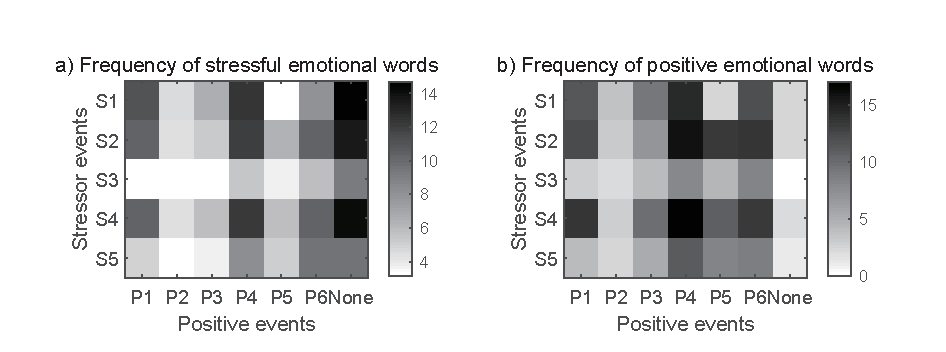
\includegraphics[width=\linewidth]{figs/gray/emotion.eps}
\caption{\small{Comparing stressful emotions and positive emotions during stressful intervals in the SI and U-SI sets.
$P_{1-6}$=\{school life, romantic relationships, peer relationships, self-cognition, family life, entertainment\},
$E_{1-5}$=\{school life, romantic relationships, peer relationships, self-cognition, family life\}.
}}
\label{fig:topicAll}
\end{figure}

 \begin{figure}[h]
\centering
\includegraphics[width=\linewidth]{figs/gray/topicOffset.eps}
\caption{\small{Offset frequency of topic words during stressful intervals in the SI and U-SI sets.
$P_{1-6}$=\{school life, romantic relationships, peer relationships, self-cognition, family life, entertainment\},
$E_{1-5}$=\{school life, romantic relationships, peer relationships, self-cognition, family life\}.}}
\label{fig:stopic}
\end{figure}

\paragraph{\textbf{Linguistic expressions}}
For each microblog, we identified its linguistic expressions
applying the segmentation model and parser model from section \ref{sec:frame1}.
The first measure was the frequency of stressful emotional words based on four categories
(anger, anxiety, hate, sad) from LICW lexicons, representing general stress during an interval~\citep{Tausczik2010The}.
The second measure was the frequency of positive emotional words,
which were identified based on the surprise, joy, expectation and love categories of the LICW lexicons.
The third measure was the frequency of topic words in the five dimensions of stressor events,
representing the degree of attention for each dimension of stressor events.
Figure \ref{fig:topicAll} (a) and (b) shows the frequency of stressful emotional words and positive emotional words, respectively.
Generally, positive events showed stress-buffering effects in these two measures,
since the last column in subgraphs (a) and (b) is different compared to columns P1 to P6.
Specifically, positive events from romantic, peer relationship and family life shows obvious
reductions in stressful emotional words caused by
peer relationship and family life stressor events (subgraph \ref{fig:topicAll} (a)).
Figure \ref{fig:stopic} shows the distribution of stressful topic words when different positive events occurred.
Here, we shows the statistical results during stressful intervals caused by school-life and self-cognition stressor events.
The frequency of stressful academic topic words (subgraphs (a1) and (b1))
and positive academic topic words (subgraphs (a2) and (b2)) shows no clear regularity.
Furthermore, we explored the offset for each dimension of stressful and positive topic words,
as shown in subgraphs (a3) and (b3).
The offset results shows obvious stress-buffering results
because stressful topic words shows a decrease in columns P1 to P5 in subgraph (a3),
and positive topic words exhibit increases in columns P1 to P5 in subgraph (b3).
These findings reveal that the occurrence of positive events offset the impact of stressor events
by simultaneously discussing positive topics.

\begin{figure}[h]
\centering
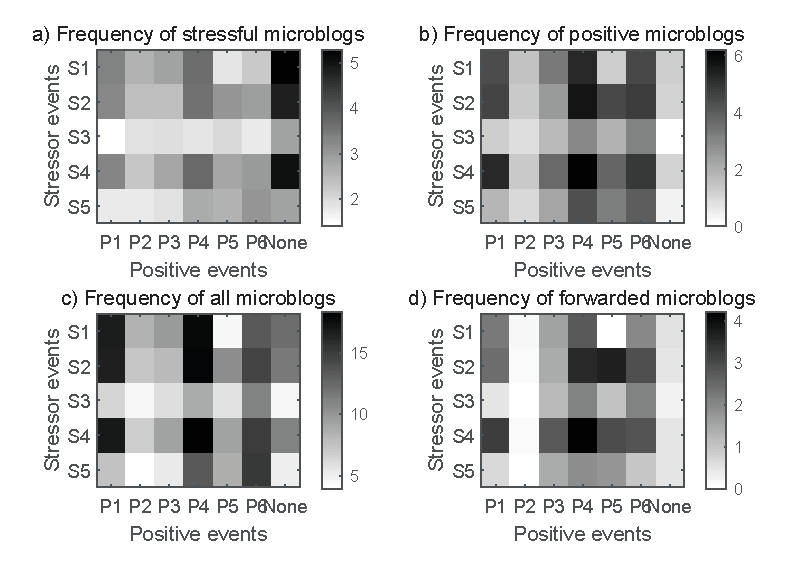
\includegraphics[width=\linewidth]{figs/gray/post.eps}
\caption{\small{Comparing posting behaviors during stressful intervals in SI and U-SI sets.
$P_{1-6}$=\{academic, romantic, peer relationship, self-cognition, family life, entertainment\},
$E_{1-5}$=\{academic, romantic, peer relationship, self-cognition, family life\}.}}
\label{fig:post}
\end{figure}

\paragraph{\textbf{Posting behaviors}}
Stress can lead to abnormal posting behaviors,
reflecting users' changes in social engagement activities~\citep{Liang2015Teenagers}.
We considered four measures of posting behaviors here.
The first measure was the frequency of stressful microblogs,
highlighting stressful microblogs among all microblogs.
Research in \cite{Li2017Analyzing} indicated that overwhelmed adolescents
tended to post more microblogs expressing their stress for release and to seek comfort from friends.
The second measure was the frequency of positive microblogs,
indicating the number of positive microblogs per day.
The third measure was the total number of all microblogs per day.
The fourth measure was the frequency of forwarded microblogs,
showing the number of retweets and shared microblogs.
Figure \ref{fig:post} summarizes the distribution of the above four measures in the U-SI and SI sets.
The results in subgraphs (a) and (b) show a decrease in stressful microblogs and
an increase in positive microblogs when positive events occurred.
Subgraph (d) indicates that adolescents tended to forward more microblogs when positive events occurred,
while subgraph (c) showed that the frequency of all microblogs did not appear to change significantly under the impact of positive events.

\begin{table*}
\begin{center}
\caption{\small{Monotonous stress intensity changes in U-SI and SI intervals compared with adjacent intervals.
 \emph{Front$ \rightarrow$ I} represented monotonous increase from the front interval to current stressful interval $I$.
\emph{I $\rightarrow$ rear} represented monotonous decrease from interval $I$ to its rear interval.
}}
%\resizebox{\textwidth}{15mm}{
\small{
\begin{tabular}{l cccccc cccccc} \\\hline
\multirow{2}{1cm}{}
&\multicolumn{2}{c}{school life}
&\multicolumn{2}{c}{romantic}
&\multicolumn{2}{c}{peer relationship}
&\multicolumn{2}{c}{self-cognition}
&\multicolumn{2}{c}{family life}
&\multicolumn{2}{c}{all types}\\
&U-SI	    &	SI	        &U-SI	    &SI	        &U-SI	   &SI	
&U-SI	    &	SI	        &	U-SI	&SI	        &U-SI	   &SI\\  \hline
\# interval         &   365	        &	514	        &	536	        &	587	        &128	    &	391	        &	564	           &	609	            &	321	        &	481	        &	1,914	    &2,582	 \\
front $\rightarrow$ I &	72.60\% &	78.79\% &	69.03\% 	&77.51\%   &74.22\%    &81.59\%    &70.04\%    &77.67\%  &67.91\%     &77.96\%    &70.17\%    &78.51\% \\
I $\rightarrow$ rear  &	75.89\% &	78.40\% &	74.63\% 	&79.05\%   &78.13\%    &82.61\%    &75.00\%    &79.15\%   &74.14\%    &79.42\%    &75.13\%    & 79.55\%\\ \hline
\end{tabular}}%}}
\label{tab:fontrear}
\end{center}
\end{table*}

\subsubsection{Monotonic Model of Stress-buffering}
\label{sec:mono}
To further verify the monotonic changes in stress intensity under the impact of positive events,
for each stressful interval in the SI (n=2,582) and U-SI (n=1,914) sets,
we compared its stress intensity with the front- and rear-adjacent intervals.
For a stressful interval $I = <t_i,t_{i+1},\cdots,t_j>$,
let $I^{front} = <t_m,\cdots,t_{i-1}>$ be the adjacent interval before $I$,
and $I^{rear} = <t_{j+1},\cdots,t_n>$ be the rear-adjacent interval of $I$.
The lengths of $I^{front}$ and $I^{rear}$ were set to $|I|$.
For the set of stressful intervals $SI$ composed of $<I_1,I_2,\cdots,I_N>$,
the corresponding sets of adjacent front and rear intervals are denoted by $SI^{front}$ and $SI^{rear}$, respectively.
Similarly, for the set of stressful intervals $USI$ = $<UI_1,UI_2,\cdots, UI_M>$ impacted by positive events,
the corresponding sets of front-adjacent intervals and rear-adjacent intervals are denoted by $USI^{front}$ and $USI^{rear}$, respectively.
We compared the intensity of stress changes in the following four situations,
where $g(.)$ is the function comparing two sets: \\
1) \small{$g(SI,SI^{front})$} is returned if a stress-intensity change occurred when a stressful interval began.\\
2) \small{$g(SI,SI^{rear})$} is returned if a stress-intensity change occurred after a stressful interval ended.\\
3) \small{$g(USI,USI^{front})$} is returned if a stress-intensity change occurred when a stressful interval affected by positive events began.\\
4) \small{$g(USI,USI^{rear})$} is returned if a stress-intensity change occurred after a stressful interval affected by positive events ended.

In our problem, taking the comparison between $SI$ and $SI^{rear}$ as an example,
the basic computation element $I_k \in SI \cup SI^{rear}$ in both sets was an interval,
represented by a multidimensional point.
Here, we adopt a t-test as the intensity computation function $g(.)$.
The function $g(.) = t_{score}$ $\in$ (-1,1) is represented as:
\begin{equation}
\small{g(SI,SI^{rear})}= \frac{\mu_{SI}-\mu_{SI^{rear}}}{\sqrt{\frac{(n_1-1)\sigma^2_{SI}+(n_2-1)\sigma^2_{SI^{rear}}}{n_1+n_2-2}(\frac{1}{n_1}-\frac{1}{n_2})}}
\end{equation}
where $\mu_{SI}$ and $\mu_{SI^{rear}}$ are the mean stress values
of intervals in sets $SI$ and $SI^{rear}$, respectively,
and $\sigma_{SI}$ and $\sigma_{SI^{rear}}$ are the variance of the stress values of the intervals in sets $SI$ and $SI^{rear}$, respectively.
If $g(SI,SI^{rear})$ $> \alpha$, the stress intensity in $SI^{rear}$ showed a significant decrease compared with $SI$ (monotonic negative effect).
If $g(SI^{front},SI)$ $< -\alpha$, the stress intensity in $SI$ showed a significant increase compared with $SI^{front}$ (monotonic positive effect).
Here, we adopted $\alpha$ = 1.96; $P$ = 0.025.
We conducted a comparison for the above four situations
to observe whether the occurrence of positive events relieved the monotonic negative effect of $g(SI,SI^{rear})$
and the monotonic positive effect of $g(SI^{front},SI)$.
